\documentclass[11pt]{article}
% General document formatting
\usepackage[margin=0.75in]{geometry}
\usepackage[parfill]{parskip}
\usepackage[utf8]{inputenc}
\usepackage{subfig}         % side-by-side figures 
% Related to math
\usepackage{amsmath,amssymb,amsfonts,amsthm}
\usepackage{graphicx}
\usepackage{natbib}
\usepackage{titling}
\usepackage{hyperref}
\usepackage{wrapfig}
\usepackage{booktabs} % for wrapping tabulars in accord with
\bibliographystyle{agu}
\setlength{\droptitle}{-5em}   % This is your set screw

%\usepackage[math]{kurier}
\newcommand\be{\begin{equation}} % shortcut to start eq envs 
\newcommand\ee{\end{equation}}   % shortcut to end eq envs
\newcommand\bra{\langle}
\newcommand\ket{\rangle}
\begin{document}

\title{Bedload diffusion theory}
\author{Kevin Pierce}
\maketitle
\begin{wrapfigure}{r}{0.45\textwidth}
	\centering
	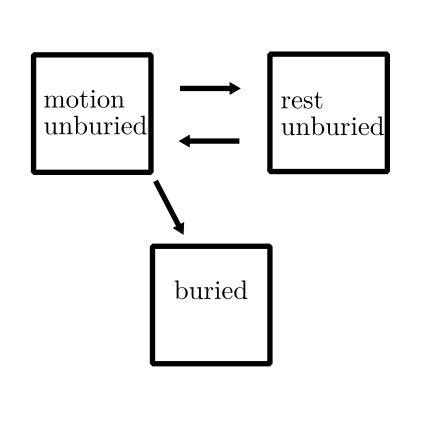
\includegraphics[width=0.3\textwidth,keepaspectratio]{diagram.png}
	\caption{Schematic depiction of the three state process}
	\label{fig:schematic}
\end{wrapfigure}
I consider a three-state random walk to describe the diffusion of sediment tracers undergoing burial within a river channel.
The first state is motion, the second is resting on the bed, and the third is burial.



Let $\omega_2(x,t)$ be the probability that an (unburied) tracer just transitioned into motion having position $x$ at time $t$, and let $\omega_1(x,t)$ be the probability that an unburied tracer just transitioned to rest having position $x$ at time $t$.
Suppose unburied tracers become buried tracers with constant probability $\kappa$ per time.
Then the probability a tracer does not become buried after resting for duration $t$ is \be\Phi(t) = e^{-\kappa t}.\ee
\vspace{2cm}

\section{Probabilities that a transition just occurred}
Let the initial probabilities for a tracer being at rest or in motion be $\theta_1$ and $\theta_2$; let $\omega_1(x,t)$ be the joint distribution of finding the particle trapped at $x,t$ just at the completion of a rest sojourn; let $\omega_1(x,t)$ be the joint distribution of finding the particle free at $x,t$ just at the completion of a rest sojourn; and let $\omega_2(x,t)$ be the joint distribution to find the tracer at $x,t$ just at the completion of a motion sojourn.
Using arguments analogous to the two-state random walk \citep[e.g.][]{Weiss1976,Weiss1994} and to reaction-diffusion problems \citep[e.g.][]{Schmidt2007}, we have 
\begin{align}
\omega_1(x,t) &= \theta_1 g_1(x,t)\Phi(t) + \int_0^t dt' \int_0^x dx' \omega_2(x',t')\Phi(t-t')g_1(x-x',t-t'), \\
\sigma_1(x,t) &= \theta_1 g_1(x,t)\big[1-\Phi(t)\big] + \int_0^t dt' \int_0^x dx' \omega_2(x',t')\big[1-\Phi(t-t')\big]g_1(x-x',t-t'), \\
\omega_2(x,t) &= \theta_2g_2(x,t) + \int_0^t dt' \int_0^x dx' \omega_1(x',t')g_2(x-x',t-t')
\end{align}
The double laplace transforms are 
\begin{align}
\hat{\omega}_1(\eta,s) &= \theta_1 \hat{g}_1(\eta,s) \\
\hat{\sigma}_1(\eta,s) &= \theta_1\big[\hat{g}_1(\eta,s) - \hat{g}_1(\eta,s+\kappa)\big] -\\
\hat{\omega}_2(\eta,s) &= \theta_2 \hat{g}_2(\eta,s) \\
\end{align}
and this now purely algebraic system has solutions
\begin{align}
\hat{\omega}_0 &=\frac{\theta_1\hat{g}_1(\eta,s) + \theta_2\hat{g}_1(\eta,s) \hat{g}_2(\eta,s)}{1- \hat{g}_1(\eta,s)\hat{g}_2(\eta,s+\kappa)}\big[\hat{g}_0(\eta,s)-\hat{g}_0(\eta,s+\kappa)\big]  \\
\hat{\omega}_1 &= \frac{\theta_1\hat{g}_1(\eta,s) + \theta_2\hat{g}_1(\eta,s) \hat{g}_2(\eta,s)}{1- \hat{g}_1(\eta,s)\hat{g}_2(\eta,s+\kappa)} \\
\hat{\omega}_2 &= \frac{\theta_2 \hat{g}_2(\eta,s)  + \theta_1 \hat{g}_1(\eta,s)\hat{g}_2(\eta,s+\kappa)}{1- \hat{g}_1(\eta,s)\hat{g}_2(\eta,s+\kappa)}
\end{align}

\section{Probabilities away from transition points}
Define 
\be G_i(x,t) = f_j(x,t)\Psi_i(t)\ee
where $\Psi_i(t) = \int_t^\infty \psi_i(t)dt$.
This is the probability density that a sojourn in state $i$ lasts longer than time $t$ and the walker undergoes a displacement $x$ during this time.
Denote by $p_i(x,t)$ the probability that a tracer is found in state $i$ having position $x$ and $t$. These are related to the $\omega_i(x,t)$ by 
\begin{align}
p_0(x,t) &= \int_0^x dx' \int_0^t dt' \omega_1(x',t')\big[1-\Phi(t-t')\big]G_0(x-x',t-t')\\
 p_1(x,t) &= \theta_1 G_1(x,t) +\int_0^x dx' \int_0^t dt' \omega_2(x',t') G_1(x-x',t-t') \\
 p_2(x,t) &= \theta_2 G_2(x,t) +\int_0^x dx' \int_0^t dt' \omega_1(x',t')\Phi(t-t')G_2(x-x',t-t') \\
\end{align}
The total probability to be at $x,t$ is 
\be p(x,t) = p_0(x,t) + p_1(x,t) + p_2(x,t). \ee

Taking double transforms provides
\begin{align}
\hat{p}_0(\eta,s) &= \hat{\omega}_1(\eta,s)\big[\hat{G}_0(\eta,s) - \hat{G}_0(\eta,s+\kappa)\big] \\
\hat{p}_1(\eta,s) &= \theta_1 \hat{G}_1(\eta,s) + \hat{\omega}_2(\eta,s)\hat{G}_1(\eta,s)\\
\hat{p}_2(\eta,s) &= \theta_2 \hat{G}_2(\eta,s) + \hat{\omega}_1(\eta,s)\hat{G}_2(\eta,s+\kappa)\\
\end{align}
The total probability is
\be p(x,t) = \ee






\section{Propagators}
In all cases, $g_0(x,t) = \delta(x)\theta(t)$, reflecting the fact that buried tracers do not move and so are equally probable to be found at any future time exclusively at the location $x$.
The other propagators $g_1$ and $g_2$ have been previously considered by \citet{Einstein1937} and \citet{Lisle1998}.
Einstein's propagators are $g_1(x,t) = \delta(x)k_1e^{-k_1t}$ and $g_2(x,t) = k_2e^{-k_2 x}\delta(t)$ reflecting instantaneous steps and exponentially distributed steps and rests of characteristic scales $k_1$ and $k_2$.
Lisle's propagators are $g_1(x,t) = \delta(x)k_1e^{-k_1t}$ and $g_2(x,t) = \delta(x-vt)k_2e^{-k_2t}$ reflecting motions of characteristic timescale $k_1$ having velocity $v$ and rests having characteristic timescale $k_2$.
\subsection{Einstein propagators}
Einstein's assumptions in the double transformed representation are
\begin{align}
\hat{g}_0(\eta,s) &= \frac{1}{s} \\
\hat{g}_1(\eta,s) &= \frac{k_1}{k_1+s}\\
\hat{g}_2(\eta,s) &= \frac{k_2}{k_2 + \eta}\\
\end{align}
and because of the exponential sojourn times, 
\begin{align}
\hat{G}_0(\eta,s) &= \\
\hat{G}_1(\eta,s) &= \frac{1}{k_1 + s}\\
\hat{G}_2(\eta,s) &= \frac{1}{k_2 + \eta}\\
\end{align}
\subsection{Lisle propagators}
Lisle's are similarly
\begin{align}
\hat{g}_0(\eta,s) &= \frac{1}{s}\\
\hat{g}_1(\eta,s) &= \frac{k_1}{k_1+s}\\
\hat{g}_2(\eta,s) &= \frac{k_2}{k_2 + \eta v + s}
\end{align}
and
\begin{align}
\hat{G}_0(\eta,s) &= \\
\hat{G}_1(\eta,s) &= \frac{1}{k_1 + s}\\
\hat{G}_2(\eta,s) &= \frac{1}{k_2 + \eta v+ s}\\
\end{align}






\bibliography{biblio}
\end{document}



